\chapter{Test of input and output impedance of the TS464 operational amplifier}
\label{app:opamp_impedance}

The test was made to measure the input- and output- impedance of the TS464 \gls{opamp}. \\

\section{Material and Setup}

In order to perform this test, the following material has been used:

\begin{itemize}
	\item TS464 operational amplifier
	\item Analog Discovery Digilent 2 USB Oscilloscope
	\item A computer with Waveforms 2015 and MATLAB
	\item Wires
\end{itemize}


At first the input impedance will be measured, using the setup in \autoref{fig:opamp_zi}, where $R_S$ is chosen \SI{1}{\mega\ohm}. Afterwords the output impedance will be measured, using the setup in \autoref{fig:opamp_zo}, where $R$ is set to \SI{1}{\kilo\ohm}. In both cases $V_S$ is set to make a \SI{1}{\kilo\hertz} sine, with an amplitude of \SI{0.5}{\volt} and a \SI{2}{\volt} offset.

\begin{figure}[h!]
\centering
\begin{circuitikz}\draw (0,0)
(3,.5) node[op amp]{}
(-1,0)to[R=$R_S$] (1,0)
(1,0)to[short]  (2,0)
(4,.5)to[short] (5,.5)
to[short] (5,2)
to[short] (1,2)
to[short] (1,1)
to[short] (2,1)
(-1,0)to[short](-1.5,0)
to[sV=$V_S$] (-1.5,-2)
node[ground]{}
(1,0)to[sV=$V_2$] (1,-2)
node[ground]{}
(5,.5)to[R=$R_L$] (5,-2)
node[ground]{}

;\end{circuitikz}
\caption{Test setup for measuring input impedance of an \gls{opamp}, where $R_S =$\SI{1}{\mega\ohm} and $R_L = $\SI{1}{\kilo\ohm}.}
\label{fig:opamp_zi}
\end{figure}

\begin{figure}[h!]
\centering
\begin{circuitikz}\draw (0,0)
(3,.5) node[op amp]{}
(-1,0)to[R=$R_S$] (1,0)
(1,0)to[short]  (2,0)
(4,.5)to[short] (5,.5)
to[short] (5,2)
to[short] (1,2)
to[short] (1,1)
to[short] (2,1)
(-1,0)to[short](-1.5,0)
to[short] (-1.5,-2)
node[ground]{}
(5,.5)to[R=$R_L$] (7.5,.5)
to[sV=$V_S$] (7.5,-2)
node[ground]{}
(5,.5)to[sV=$V_2$] (5,-2)
node[ground]{}

;\end{circuitikz}
\caption{Test setup for measuring output impedance of an \gls{opamp}, where $R_S = R_L = $\SI{1}{\kilo\ohm}.}
\label{fig:opamp_zo}
\end{figure}



\section{Test Procedure}

For the input impedance the steps are as follows:
\begin{itemize}
\item Measure the amplitude of the signal at $V_S$.
\item Measure the amplitude of the signal at $V_2$ 
\item Subtract $V_2$ from $V_S$ to get the amplitude of $V_1$. 
\item Use \autoref{eq:opamp_zi} to calculate the input impedance.
\end{itemize}

\begin{equation}\label{eq:opamp_zi}
        Z_i = \frac{V_2}{V_1} \cdot R_S
        \addunit{\si{\ohm}}
    \end{equation}

    \startexplain
        \explain{$Z_i$ is the input impedance of the \gls{opamp}}{\si{\ohm}}
        \explain{$V_2$ is the voltage over the input of the \gls{opamp}}{\si{\volt}}
        \explain{$V_1$ is the voltage $R_S$}{\si{\volt}}
    \stopexplain
    
For the output impedance the steps are as follows:
\begin{itemize}
\item Measure the amplitude of the signal at $V_S$.
\item Measure the amplitude of the signal at $V_2$ 
\item Subtract $V_2$ from $V_S$ to get the amplitude of $V_1$. 
\item Use \autoref{eq:opamp_zo} to calculate the input impedance.
\end{itemize}

\begin{equation}\label{eq:opamp_zo}
        Z_o = \frac{V_2}{V_1} \cdot R
        \addunit{\si{\ohm}}
    \end{equation}

    \startexplain
        \explain{$Z_o$ is the output impedance of the \gls{opamp}}{\si{\ohm}}
        \explain{$V_2$ is the voltage over the output of the \gls{opamp}}{\si{\volt}}
        \explain{$V_1$ is the voltage $R$}{\si{\volt}}
    \stopexplain

\section{Results}

In \ref{fig:opamp_zi_v0} the measurement of $V_S$, when measuring the input impedance shown, and in \ref{fig:opamp_zi_v2} the measurement of $V_2$, when measuring the input impedance shown. \\

\begin{figure}[hbt]
  \centering
  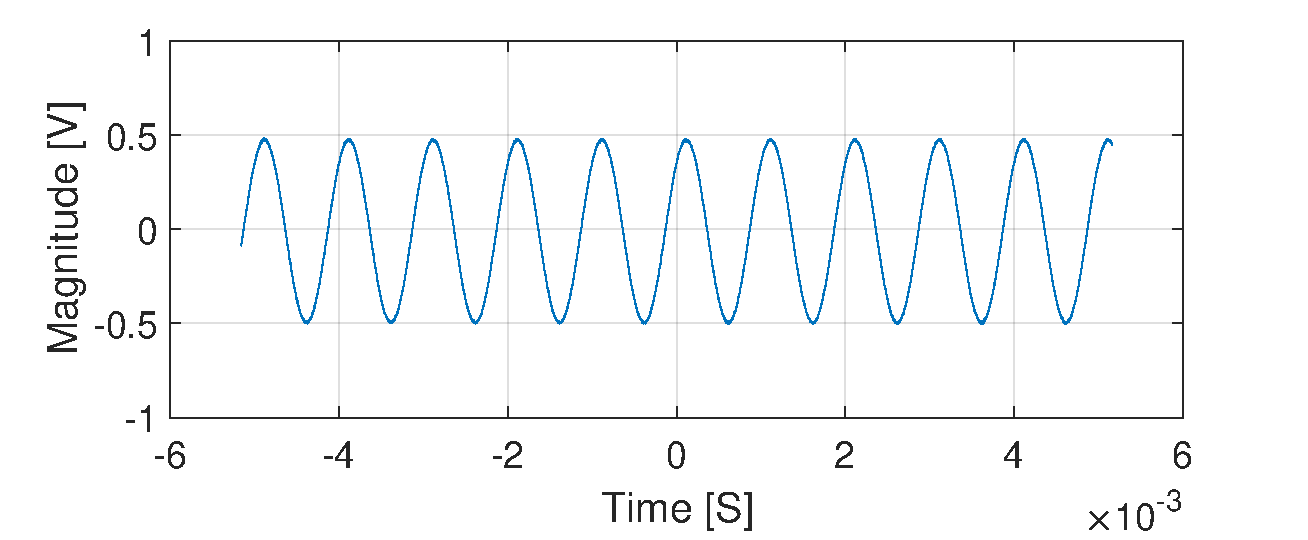
\includegraphics[width=1\textwidth]{opamp_zi_v0}
  \caption{Measurement of $V_S$, when measuring the input impedance.}
  \label{fig:opamp_zi_v0}
\end{figure}

\begin{figure}[hbt]
  \centering
  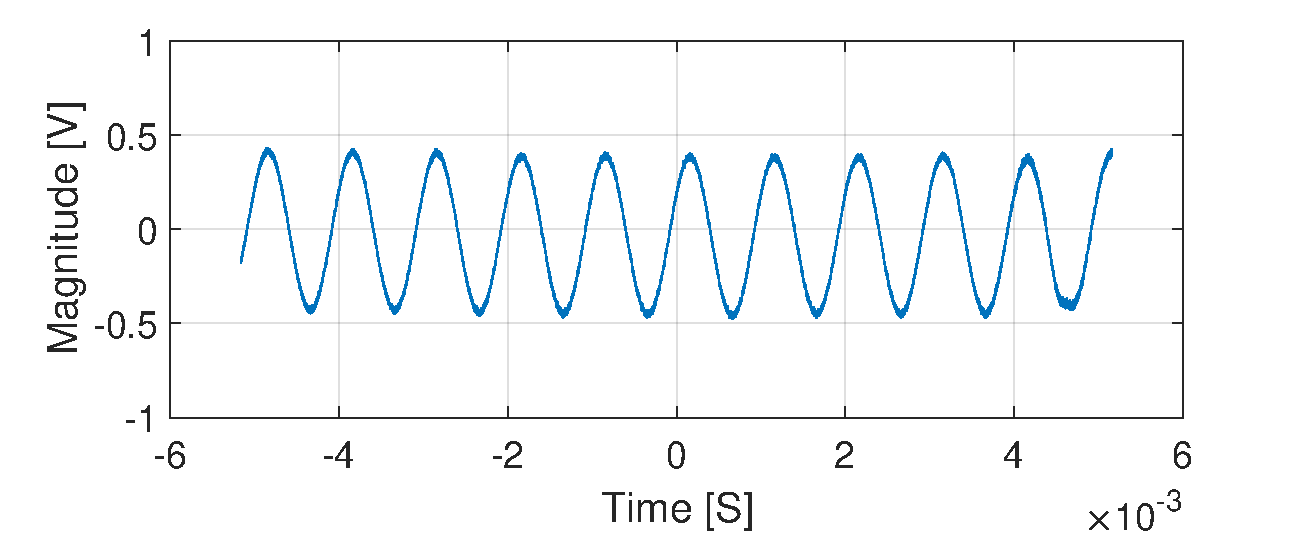
\includegraphics[width=1\textwidth]{opamp_zi_v2}
  \caption{Measurement of $V_2$, when measuring the input impedance.}
  \label{fig:opamp_zi_v2}
\end{figure}

In \ref{fig:opamp_zo_v0} the measurement of $V_S$, when measuring the output impedance shown, and in \ref{fig:opamp_zo_v2} the measurement of $V_2$, when measuring the output impedance shown. \\

\begin{figure}[hbt]
  \centering
  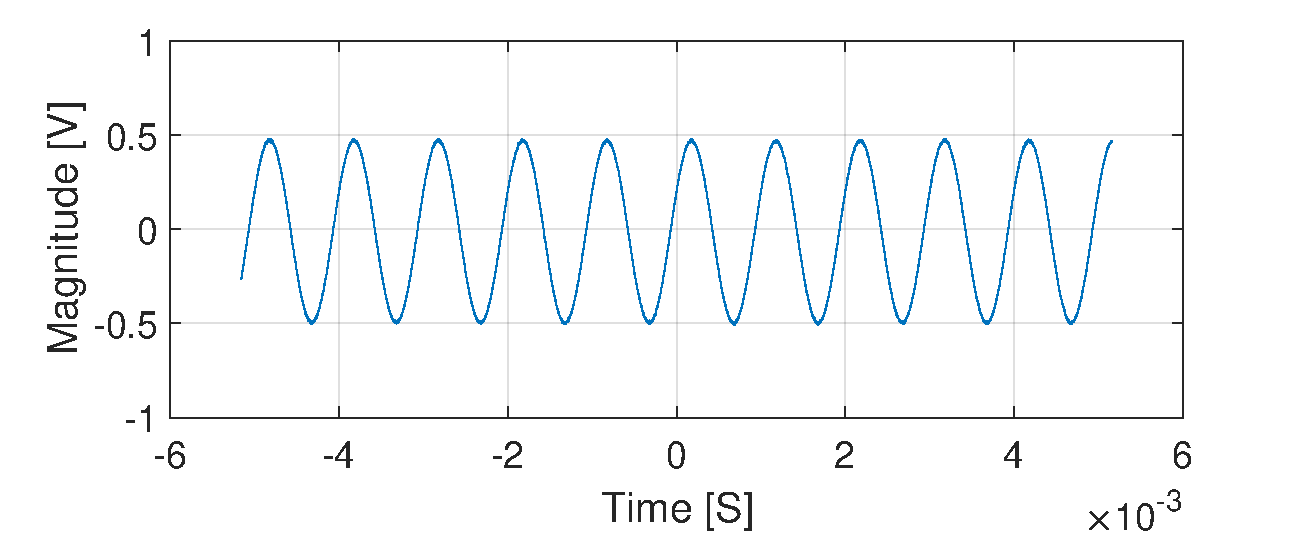
\includegraphics[width=1\textwidth]{opamp_zo_v0}
  \caption{Measurement of $V_S$, when measuring the output impedance.}
  \label{fig:opamp_zo_v0}
\end{figure}

\begin{figure}[hbt]
  \centering
  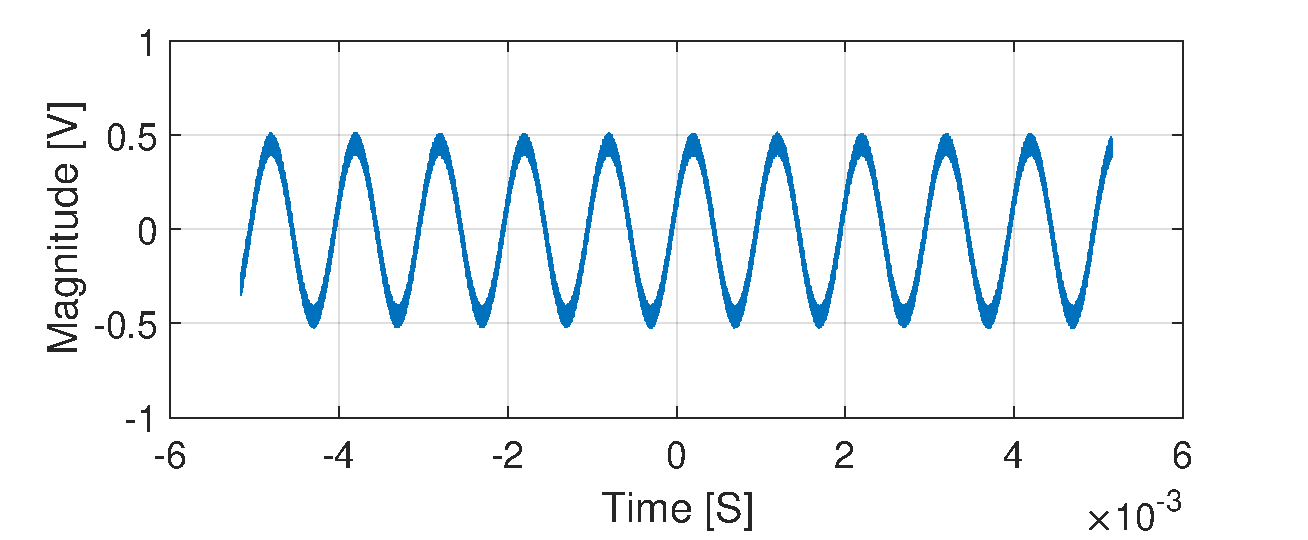
\includegraphics[width=1\textwidth]{opamp_zo_v2}
  \caption{Measurement of $V_2$, when measuring the output impedance.}
  \label{fig:opamp_zo_v2}
\end{figure}

The amplitudes of $V_S$ and $V_2$, when measuring the input impedance are measured to \SI{489}{\milli\volt} and \SI{441}{\milli\volt}. $V_1$ here by is calculated to \SI{48}{\milli\volt}. The input impedance of the \gls{opamp} is therefore as in \autoref{}.

\begin{equation}\label{eq:opamp_zi}
        Z_i = \frac{441}{48} \cdot 10^6 = 9.18
        \addunit{\si{\mega\ohm}}
    \end{equation} 
    
The amplitudes of $V_S$ and $V_2$, when measuring the output impedance are measured to \SI{493}{\milli\volt} and \SI{444}{\milli\volt}. $V_1$ here by is calculated to \SI{49}{\milli\volt}. The input impedance of the \gls{opamp} is therefore as in \autoref{}.

\begin{equation}\label{eq:opamp_zo}
        Z_o = \frac{444}{49} \cdot 10^3 = 9.06
        \addunit{\si{\kilo\ohm}}
    \end{equation} 